\documentclass[usenames,dvipsnames, xcolor=table]{beamer}

\usetheme{CambridgeUS}
\usecolortheme{rose}
\addtobeamertemplate{navigation symbols}{}{%
    \usebeamerfont{footline}%
    \usebeamercolor[fg]{footline}%
    \hspace{1em}%
    \insertframenumber/\inserttotalframenumber
}

\usepackage{comment}

%\bibliographystyle{jmr}
\usepackage[style=authoryear]{biblatex}
%\bibliography{ref}
%\usepackage[authordate,bibencoding=auto,strict,backend=biber,natbib]{biblatex-chicago}

\usepackage{tikz}
\usepackage{multirow}
\usepackage{graphics}

\setbeamertemplate{button}{\tikz
  \node[
  inner xsep=5pt,
  draw=structure!90,
  fill=structure!50,
  rounded corners=4pt] {\insertbuttontext};}

\newtheorem*{remark}{Remark}
\setbeamertemplate{items}[default]
%% Language and font encodings

%%%%%%%%%%%%%%%%%%%% ABBREVIATIONS %%%%%%%%%%%%%%%%%%%%
\newcommand{\bb}[1]{\mathbb{#1}}
\renewcommand{\bf}[1]{\boldsymbol{\mathbf{#1}}}
\renewcommand{\cal}[1]{\mathcal{#1}}
\renewcommand{\frak}[1]{\mathfrak{#1}}

\newcommand{\quation}[1]{\begin{equation*}#1\end{equation*}}
\newcommand{\lign}[1]{\begin{align*}#1\end{align*}}
\newcommand{\lignat}[2]{\begin{alignat*}{#1}#2\end{alignat*}}
\newcommand{\ather}[1]{\begin{gather*}#1\end{gather*}}
\newcommand{\ultline}[1]{\begin{multline*}#1\end{multline*}}
\newcommand{\ases}[1]{\begin{cases}#1\end{cases}}

\newcommand{\obar}[1]{\overline{#1}}
\newcommand{\ubar}[1]{\underline{#1}}

\newcommand{\set}[1]{\left\{#1\right\}} % {abc} % braces
\newcommand{\pa}[1]{\left(#1\right)} % (abc) % parentheses
\newcommand{\ang}[1]{\left<#1\right>} % <abc> % angle brackets
\newcommand{\bra}[1]{\left[#1\right]} % [abc] % brackets
\newcommand{\abs}[1]{\left|#1\right|} % |abc|
\newcommand{\norm}[1]{\left\|#1\right\|} %||abc||

\newcommand{\mat}[1]{\begin{matrix}#1\end{matrix}} % \mat{1 & 0 & 1 \\ 0 & 0 & 1 \\ 1 & 1 & 0}
\newcommand{\pmat}[1]{\pa{\mat{#1}}}

\newcommand{\sm}[1]{\begin{smallmatrix}#1\end{smallmatrix}}
\newcommand{\psm}[1]{\pa{\sm{#1}}}
\newcommand{\bsm}[1]{\bra{\sm{#1}}}

\newcommand{\tci}[2]{\set{\,#1 \mid{} #2\,}}
\newcommand{\pfrac}[2]{\pa{\frac{#1}{#2}}}
\newcommand{\der}[2]{\frac{\partial #1}{\partial #2}}
\newcommand{\pder}[2]{\pfrac{\partial #1}{\partial #2}}

\newcommand{\firstp}[2]{\ensuremath{\displaystyle
     \frac{\partial{#1}}{\partial{#2}}}} % \firstp{f}{x}
\newcommand{\secondp}[3]{\ensuremath{\displaystyle
     \frac{\partial^{2}{#1}}{\partial{#2}\,\partial{#3}^T}}} % \secondp{f}{x}{y}
\newcommand{\secondpscalar}[3]{\ensuremath{\displaystyle
     \frac{\partial^{2}{#1}}{\partial{#2}\,\partial{#3}}}} % \secondp{f}{x}{y}

%%%%%%%%%%%%%%%%%%%% OPERATORS %%%%%%%%%%%%%%%%%%%%
\DeclareMathOperator{\diag}{diag}
\DeclareMathOperator{\sgn}{sgn}
\DeclareMathOperator{\tr}{tr}
\DeclareMathOperator{\SE}{SE}
\DeclareMathOperator{\Var}{Var}
\DeclareMathOperator{\Cov}{Cov}
\DeclareMathOperator{\Corr}{Corr}

\DeclareMathOperator*{\argmin}{argmin}
\DeclareMathOperator*{\argmax}{argmax}

%%%%%%%%%%%%%%%%%%%% LETTERS %%%%%%%%%%%%%%%%%%%%
\newcommand{\N}{\mathbb{N}}
\newcommand{\Z}{\mathbb{Z}}
\newcommand{\Q}{\mathbb{Q}}
\newcommand{\R}{\mathbb{R}}
\newcommand{\C}{\mathbb{C}}

\newcommand{\iidsim}{\stackrel{i.i.d.}{\sim}}
\newcommand{\iid}{\stackrel{i.i.d.}{\sim}}

\newcommand{\st}{\text{ }s.t.\text{ }}

\newcommand{\dps}{\displaystyle}

%Information to be included in the title page:

%\subtitle{Hastie, T., Tibshirani, R., Wainwright, M.\\ 
% Statistical Learning with Sparsity, Chapter 2}
\author[Kwon]{Yonghyun Kwon
\\ 
joint work with Dr. Kim}


\title[Double GREG]{  
Double GREG estimation
}
\institute{Iowa State Univeristy}
%\institute{Overleaf}

\begin{document}

\frame{\titlepage}

\section{Problem setup}

\begin{frame}{Problem setup}
\begin{itemize}
    \item Let \(A\) be a sample of size \(n\) selected from the population \(U\) of size \(N\). 
    \item Let $\pi_i$ be the first order inclusion probability of unit $i$ and $\pi_{ij}$ the second order inclusion probability of unit $i$ and $j$.
    \item Let \(y\) denote a variable of interest and we try to estimate the population total \(t_y = \sum_{i \in U} y_i\). 
    \item Let \(\bf x_{i}\) of size \(p\) be the auxiliary variables associated with \(y\). 
Assume that $\bf x_i$ is observed throughout the finite population while $y_i$ is observed only in the sample.
\end{itemize}
\end{frame}

\begin{frame}{Superpopulation model}
    \begin{itemize}
        \item Suppose the following superpopulation model holds
\begin{equation}
    y_i = \bf x_i^T \bf \beta + \varepsilon_i, \quad \varepsilon_i \iid (0,\sigma^2), \quad i = 1, \cdots, N \label{lin}
\end{equation}
\item Indeed, the linear regression model can be extended to the general nonlinear model whose basis function can be (penalized) spline functions. \eqref{lin} can be replaced by
\begin{equation}
    y_i = \sum_{j = 0}^Mh_j(\bf x_i) \beta_j + \varepsilon_i, \quad \varepsilon_i \iid (0,\sigma^2), \quad i = 1, \cdots, N 
\end{equation}
where $h_j(\cdot)$ are the corresponding basis functions. For the sake of simplicity, we assume linear basis functions in \eqref{lin} only.
    \end{itemize}
\end{frame}

\begin{frame}{GREG estimator}
    \begin{itemize}
        \item The working model \eqref{lin} motivates the GREG estimator defined by
\begin{equation}
    \hat t_y = \sum_{i \in U}\bf x_i^T \hat {\bf \beta} + \sum_{i \in A}\frac{1}{\pi_i}\pa{y_i - \bf x_i^T \hat {\bf \beta}} \label{GREG}
\end{equation}
where $\hat {\bf \beta}$ is defined by
$$
\hat {\bf \beta} = \pa{\sum_{i \in A} \frac{1}{\pi_i}\pa{\bf x_i - \bar {\bf x}}\pa{\bf x_i - \bar {\bf x}}^T}^{-1}\pa{\sum_{i \in A} \frac{1}{\pi_i}\pa{\bf x_i - \bar {\bf x}}y_i}
$$
    \end{itemize}
\end{frame}

\begin{frame}{GREG estimator}
    \eqref{GREG} enjoys many desirable design properties including:
    \begin{itemize}
        \item asymptotic equivalence to the difference estimator
        \item design consistency
        \item asymptotically design unbiasedness
        \item asymptotically normally distribution with finite variance
        \item its design variance can consistently be estimated by the linearized variance estimator
        \begin{equation}
    \hat V_p = \sum_{i,j \in A} \frac{\Delta_{ij}}{\pi_{ij}} \frac{y_i - \bf x_i \hat {\bf \beta}}{\pi_i}\frac{y_j - \bf x_j \hat {\bf \beta}}{\pi_j} \label{var}
\end{equation}
However, when the number of parameters $p$ grows as $n$ increases, the properties listed above no longer hold.
    \end{itemize}
\end{frame}

\section{Double GREG estimator}

\begin{frame}{High dimensional GREG estimator}
\begin{itemize}
    \item Now, suppose that $p$ is allowed to increase as the sample size increases.
    \item In the high-dimension setup, the estimating errors of the regression coefficients $\hat {\bf \beta}$ are no longer negligible.
    \item the GREG estimator is no longer asymptotically equivalent to the difference estimator since
$$
\hat t_{y, GREG} - \hat t_{y, diff} = 
\pa{\sum_{i \in U} \bf x_i - \sum_{i \in A}\frac{1}{\pi_i} \bf x_i } \pa{\hat {\bf \beta} - \bf \beta} \neq o_p(n^{-1}) 
$$
\item Indeed, Ta et al. (2020) recently showed that the GREG estimator is asymptotically equivalent to the difference estimator only if $p / n \to 0$.
\end{itemize}
\end{frame}

\begin{frame}{Bias of GREG estimator}
\begin{itemize}
    \item Under fixed $p$, the bias ($O(n^{-1})$) of the GREG estimator is negligible compared to its standard error($O(n^{-1/2})$) (Cochran, 1977)
    \item On the other hand, the bias of the high dimensional GREG estimator can be significant.
    \item The simulation results show that such a tendency manifests itself even stronger when the sampling design is informative (in the next section).
\end{itemize}
\end{frame}

\begin{frame}{Sample splitting}
    In this regard, we consider the sample split method. Let $A_1$ and $A_2$ be a random partition of $A$ (possibly of equal size). Let $\hat {\bf \beta}_1$ and $\hat {\bf \beta}_2$ be the generalized regression coefficients using $A_1$ and $A_2$ respectively. We propose the double GREG estimator defined as follows
    \begin{equation}
  \hat t_y = \sum_{i \in U}\bf x_i^T\tilde {\bf \beta}  + \sum_{i \in A_1} d_i \pa{y_i - \bf x_i^T \hat{\bf \beta}_2} + \sum_{i \in A_2} d_i \pa{y_i - \bf x_i^T \hat{\bf \beta}_1} \label{double}        
    \end{equation}
  where $\tilde {\bf \beta}$ is the weighted regression coefficient defined by
  \begin{equation}
        \tilde {\bf \beta} = \frac{\sum_{i \in A_2}d_i}{\sum_{i \in A}d_i} \hat{\bf \beta}_1 + \frac{\sum_{i \in A_1}d_i}{\sum_{i \in A}d_i} \hat{\bf \beta}_2 
  \end{equation}
\end{frame}

\begin{frame}{Ensemble Learning}
    \begin{itemize}
        \item Because of the random split, the resulting double GREG estimator can suffer from a large variance.
        \item In order to reduce the variance and improve efficiency, we take several random splits from a sample and take the average of all the samples.
        \item That is, for each of the random samples $A_1(1), \cdots, A_1(K)$ and $A_2(1), \cdots, A_2(K)$ the final ensemble estimator is defined as
  \begin{equation}
      \hat t_y = \frac{1}{K}\sum_{k = 1}^K \hat t_y(A_1(k), A_2(k)) \label{ensemble}
  \end{equation}
    \end{itemize}
\end{frame}

\begin{frame}{Double GREG as linear estimator}
\begin{itemize}
    \item Observe that both \eqref{double} and \eqref{ensemble} are a linear estimator of $y$.
    \item That is, the double estimator can be constructed as a weighted sum of $y$'s whose weights are not dependent on $y$. The proposed methods can be useful when multivariate $y$'s are used.
    \item If the design matrix $\bf X$ has an intercept, \eqref{double} is algebraically equivalent to
  $$
  \hat t_y = \sum_{i \in U}\bf x_i^T\tilde {\bf \beta} + \pa{\sum_{i \in A_1} d_i \bf x_i - \sum_{i \in A_2} d_i \bf x_i}^T \pa{\hat{\bf \beta}_1 - \hat{\bf \beta}_2}
  $$
\end{itemize}
\end{frame}

\section{Simulation study}

\begin{frame}{Simulation setup}
    \begin{itemize}
        \item A sample of size $n = 100$ is selected from the population of size $N = 2000$.
        \item $x_{ij} \sim N(2, 1)$
        \item Suppose the following super-population model holds \[
y_i = \bf x_i^T \bf \beta + \varepsilon_i, \quad \varepsilon_i \iid N(0,\sigma^2), i = 1, \cdots, N
\] where \(\sigma^2 = 1\) and
\(\bf \beta = (1, \cdots, 1, 0, \cdots, 0)\) with \(s =\) 20 1s and
\(p - s =\) 20 0s.
    \end{itemize}
\end{frame}

\begin{frame}{Simulation setup}
     We assume the samples are drawn from the informative stratified sampling.

    $$
    Z_j \sim Z_j^* + \varepsilon_j, \quad Z^* \sim N\pa{0, \frac{1 - r}{r}}, j \in U, r \in (0, 1)
    $$
    The finite population data $\set{y_j, \bf x_j, z_j}_{j \in U}$ are sorted by $z_j$ so that the 500 smallest $z$ values are in stratum one and the next 500 smallest value are in stratum two and so forth. Within each stratum, simple random samples are collected with size
    $$
    n_1 = 15, n_2 = 20, n_3 = 30, n_4 = 35
    $$
    The larger $r$ is, the more informative sampling design we have. We consider the following estimators. Here, we set $r = 0.75$.
\end{frame}

\begin{frame}{Simulation results}
\begin{table}[]
\begin{tabular}{crrr}
\hline
              & \multicolumn{1}{c}{BIAS} & \multicolumn{1}{c}{SE} & \multicolumn{1}{c}{RMSE} \\ \hline
HT            & 14.17                    & 344.56                 & 344.85                   \\
Diff          & -0.08                    & 118.29                 & 118.29                   \\
GREG          & 218.85                   & 198.73                 & 295.62                   \\
Double\_GREG  & 3.80                     & 240.60                 & 240.63                   \\
Lasso         & 161.60                   & 181.59                 & 243.08                   \\
Double\_Lasso & 12.39                    & 198.25                 & 198.64                   \\ \hline
\end{tabular}
\caption{}
\label{tab:my-table}
\end{table}
\end{frame}

\begin{frame}{Comparison of the estimators $\hat t_y$}
    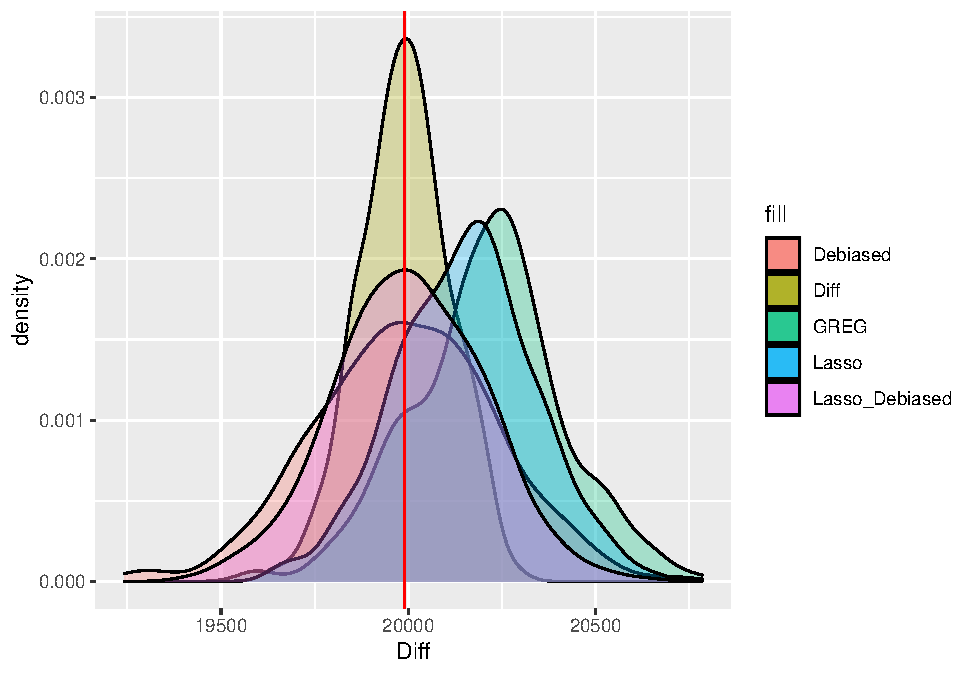
\includegraphics[width = \columnwidth]{sim/sim_092922_files/figure-latex/unnamed-chunk-3-1.pdf}
\end{frame}

\begin{frame}[t,allowframebreaks]
  \frametitle{References}
  \printbibliography
 \end{frame}

\end{document}
